\documentclass[11pt,letterpaper]{article}
\usepackage{fontspec}
\setmainfont{texgyrepagella}[Extension=.otf,UprightFont=*-regular,BoldFont=*-bold,ItalicFont=*-italic,BoldItalicFont=*-bolditalic]
\usepackage[bidi=default]{babel}
\babelprovide[import,main]{spanish}
\babelprovide[import]{hebrew}
\babelprovide[import]{ancientgreek}
\babelfont[hebrew]{rm}[Path=fonts/,BoldFont=NotoHebrewSerif-700.ttf,Scale=0.95]{NotoHebrewSerif-400.ttf}
\babelfont[ancientgreek]{rm}[Path=fonts/]{GFSPorson.otf}
\newcommand{\heb}[1]{\mbox{\foreignlanguage{hebrew}{#1}}}
\newcommand{\grc}[1]{\foreignlanguage{ancientgreek}{#1}}
\newcommand{\hebverso}[1]{\par\smallskip{\centering\begin{otherlanguage}{hebrew}\large #1\end{otherlanguage}\par}\smallskip}
\newcommand{\SENOR}{\textsc{Señor}}
\usepackage[margin=2.5cm,headheight=14pt]{geometry}
\usepackage{microtype,ragged2e,booktabs,graphicx,xcolor,csquotes,array}
\usepackage[hidelinks]{hyperref}\usepackage{xurl}\urlstyle{same}
\usepackage[most]{tcolorbox}
\usepackage{tikz}\usetikzlibrary{arrows.meta,positioning,calc,decorations.pathreplacing}
\usepackage{titlesec,fancyhdr}
\definecolor{azul}{HTML}{15437C}\definecolor{azuloscuro}{HTML}{0B1F3A}\definecolor{celeste}{HTML}{5694D6}
\definecolor{dorado}{RGB}{196,154,60}\definecolor{papiro}{RGB}{246,239,220}\definecolor{gris}{RGB}{70,78,96}
\titleformat{\section}{\Large\bfseries\color{azul}}{\thesection.}{0.6em}{}
\titleformat{\subsection}{\large\bfseries\color{azuloscuro}}{\thesubsection}{0.6em}{}
\pagestyle{fancy}\fancyhf{}
\fancyhead[L]{\foreignlanguage{spanish}{\small\itshape\color{gris}Dios es amor}}\fancyhead[R]{\foreignlanguage{spanish}{\small\color{gris}\thepage}}
\renewcommand{\headrulewidth}{0.4pt}
\setlength{\parindent}{1.27cm}\linespread{1.15}\setlength{\emergencystretch}{3em}
\newtcolorbox{cita}[1][]{enhanced,colback=azul!6!white,colframe=azul,boxrule=0pt,leftrule=2.5pt,arc=0pt,
  left=8pt,right=8pt,top=5pt,bottom=5pt,before skip=8pt,after skip=8pt,fontupper=\itshape,#1}
\newcommand{\fuente}[1]{\par\hfill{\upshape\bfseries\small\textcolor{azul}{#1}}}
\newtcolorbox{nota}[1][]{enhanced,colback=dorado!10,colframe=dorado!85!azul,boxrule=0.6pt,arc=2pt,
  fonttitle=\bfseries\small,coltitle=azuloscuro,colbacktitle=dorado!30,fontupper=\small,title={#1}}
\newtcolorbox{filologia}[1][]{enhanced,colback=white,colframe=azul!45,boxrule=0.5pt,arc=2pt,
  fonttitle=\bfseries\small,coltitle=white,colbacktitle=azul!80,fontupper=\small,title={Filología: #1}}
\newcommand{\refapa}[1]{\par{\RaggedRight\hangindent=1.27cm\hangafter=1\noindent #1\par}\vspace{4pt}}
\newcommand{\destacar}[1]{\textbf{\textcolor{azul}{#1}}}
\newcolumntype{L}[1]{>{\RaggedRight\arraybackslash}p{#1}}


\title{\color{azul}\bfseries Dios es amor\\[4pt]\large\color{gris}\mdseries Un amor eterno, soberano e inmutable (1 Jn 4:7--16)}
\author{}\date{}
\begin{document}
\maketitle\thispagestyle{empty}

\begin{abstract}\noindent
``Dios es amor'' (1 Jn 4:8, 16) es una de las tres frases con que la Escritura declara qué es Dios; las otras dos son ``Dios es Espíritu'' (Jn 4:24) y ``Dios es luz'' (1 Jn 1:5). Esa es la razón de que esta serie sitúe el amor entre los atributos del Ser. El capítulo parte de 1 Juan 4:7--16 y sigue el eje propuesto por el autor de la serie: el amor de Dios es \emph{eterno} (Jer 31:3), \emph{soberano} (Dt 7:7--8; Mal 1:2) e \emph{inmutable} (Mal 3:6; Os 11:8--9). Estudia la raíz hebrea \emph{ahav}, con sus cerca de 250 apariciones, desde su primera vez en Génesis 22:2 y desde el lenguaje de pacto de Deuteronomio; recorre después las demás palabras que la Reina-Valera traduce ``amor'', ``amar'' o ``amado'' (713 veces en 608 versículos, según conteo propio) y la familia griega de \emph{agapē} y \emph{phileō}. El encuentro en la historia de Israel es Oseas, a quien Dios manda amar a una adúltera ``como el amor del \SENOR{} para con los hijos de Israel''. La lectura judía recoge el Shemá y sus bendiciones (\emph{Ahavá rabbá}, \emph{Ahavat olam}), la Misná, el Sifré, el martirio de Rabí Akiva, los targumes, Rashi y Maimónides. La lectura paulina encuentra ese mismo amor en la cruz: derramado (Ro 5:5), demostrado (Ro 5:8), inseparable (Ro 8:35--39), anterior a la fundación del mundo (Ef 1:4--6) y personal (Gá 2:20).
\par\smallskip\noindent\textbf{Palabras clave:} amor, \emph{ahav}, \emph{ahavá}, \emph{agapē}, 1 Juan 4, Deuteronomio 7, Oseas, Shemá, Pablo.\end{abstract}

\begin{nota}[Nota sobre el texto]
Las citas bíblicas proceden de la Reina-Valera 1960. Donde esta escribe ``Jehová'', aquí se escribe \SENOR, que traduce el tetragrama \heb{יהוה}, leído en la tradición judía como \emph{Adonay}. El hebreo sigue la BHS; el griego, NA28 y la Septuaginta de Rahlfs-Hanhart. Las fuentes judías (Misná, Talmud, Sifré, Rashi, targumes, Maimónides) se citan desde Sefaria y se marcan como precisión; cuando no existe traducción española publicada, la traducción es propia. Si la numeración hebrea difiere de la española, se indica entre corchetes. El autor de la serie aportó el texto ancla (1 Jn 4:7--16) y el eje del capítulo, un amor \emph{eterno, soberano e inmutable}; el resto es una base propuesta para su revisión.
\end{nota}

%===================================================================
\section{Un atributo del ser}

Pocas palabras se usan tanto y se entienden tan poco como ``amor''. En el habla de hoy nombra, casi siempre, un sentimiento intenso, espontáneo y cambiante; aplicada a Dios, suele degradarse en una indulgencia que lo tolera todo. Pink advertía que muchos hablan del amor de Dios sin conocer al Dios de amor, y que la idea corriente lo reduce a una emoción blanda, modelada según la nuestra (Pink, 2020, cap.~16). La Escritura no corrige ese error con una definición abstracta. Lo corrige con tres afirmaciones sobre lo que Dios \emph{es}:

\begin{center}\small\renewcommand{\arraystretch}{1.2}
\begin{tabular}{@{}L{3.6cm}L{3.0cm}L{8.2cm}@{}}
\toprule
\textbf{Afirmación} & \textbf{Texto} & \textbf{Lo que dice de Dios} \\ \midrule
``Dios es Espíritu'' & Jn 4:24 & Su modo de ser: no está limitado a un lugar ni a un cuerpo. \\
``Dios es luz'' & 1 Jn 1:5 & Su pureza: ``no hay ningunas tinieblas en él''. \\
``Dios es amor'' & 1 Jn 4:8, 16 & Su vida misma: el amor no es algo que Dios tenga, sino lo que es. \\
\bottomrule
\end{tabular}\par
{\footnotesize\color{gris}\textit{Tabla 1.} Las tres afirmaciones ``Dios es''. \textit{Nota.} Elaboración propia a partir de Pink (2020, cap.~16).}
\end{center}

De ahí que esta serie coloque el amor entre los atributos del \destacar{Ser}, junto a la unidad y la espiritualidad. Decir que Dios ama describe lo que hace; decir que Dios \emph{es} amor describe lo que es antes de hacer cosa alguna, antes de que existiera una criatura a quien amar. Pink lo formula con precisión: ``No es simplemente que Dios `ama', sino que Él es el amor mismo. El amor no es meramente uno de sus atributos, sino su propia naturaleza'' (Pink, 2020, p.~83).

\begin{nota}[Precisión]
Clasificación propuesta: atributo del Ser. Es \emph{incomunicable} en su plenitud, porque solo el amor de Dios es eterno, sin causa fuera de sí e invariable, y \emph{comunicable} como reflejo: ``Amados, si Dios nos ha amado así, debemos también nosotros amarnos unos a otros'' (1 Jn 4:11). Queda sujeta a la revisión del autor de la serie.
\end{nota}

El autor de esta serie resumió el atributo en tres palabras: el amor de Dios es \destacar{eterno}, \destacar{soberano} e \destacar{inmutable}. Las tres responden a una misma pregunta mirada desde ángulos distintos. ¿Cuándo empezó ese amor? Nunca: es eterno. ¿Qué lo causó? Nada fuera de Dios: es soberano. ¿Puede acabar? No: es inmutable. El capítulo sigue los tres rasgos en los textos hebreos y en Pablo, y de ellos se desprende que ese amor es también santo y que en Cristo se revela infinito y lleno de gracia (Ef 3:19; Ro 8:32).

\begin{center}\small\renewcommand{\arraystretch}{1.2}
\begin{tabular}{@{}L{2.4cm}L{4.6cm}L{4.0cm}L{3.8cm}@{}}
\toprule
\textbf{Rasgo} & \textbf{Pregunta} & \textbf{Texto hebreo} & \textbf{Texto paulino} \\ \midrule
Eterno & ¿Cuándo empezó? & ``Con amor eterno te he amado'' (Jer 31:3) & ``antes de la fundación del mundo'' (Ef 1:4--5) \\
Soberano & ¿Qué lo causó? & ``No por ser vosotros más\ldots{} sino por cuanto el \SENOR{} os amó'' (Dt 7:7--8) & ``según el puro afecto de su voluntad'' (Ef 1:5); ``A Jacob amé'' (Ro 9:13) \\
Inmutable & ¿Puede acabar? & ``Yo \SENOR{} no cambio'' (Mal 3:6); ``¿Cómo podré abandonarte?'' (Os 11:8) & ``nada nos podrá separar'' (Ro 8:38--39) \\
\bottomrule
\end{tabular}\par
{\footnotesize\color{gris}\textit{Tabla 2.} El eje del capítulo. \textit{Nota.} Elaboración propia.}
\end{center}

%===================================================================
\section{Texto ancla: 1 Juan 4:7--16}

\subsection{El contexto}
Juan escribe a iglesias sacudidas por maestros que habían salido de la comunidad y negaban que Jesús fuera el Cristo venido en carne (1 Jn 2:18--19, 22; 4:1--3). Frente a ellos, la carta ofrece tres pruebas de la vida verdadera: creer que Jesús es el Hijo de Dios, obedecer sus mandamientos y amar a los hermanos. Cuando llega al capítulo 4, la tercera prueba descansa sobre la teología más alta de toda la carta: el amor entre hermanos no es una virtud social, sino que brota de lo que Dios es.

\begin{nota}[Precisión]
1 Juan no es una carta de Pablo. Se adopta como texto ancla porque contiene la afirmación ``Dios es amor'' y porque así lo pidió el autor de la serie. La lectura paulina del atributo se desarrolla en la sección~\ref{sec:cristo-amor}.
\end{nota}

\subsection{El texto}
\begin{cita}Amados, amémonos unos a otros; porque el amor es de Dios. Todo aquel que ama, es nacido de Dios, y conoce a Dios. El que no ama, no ha conocido a Dios; porque Dios es amor. En esto se mostró el amor de Dios para con nosotros, en que Dios envió a su Hijo unigénito al mundo, para que vivamos por él. En esto consiste el amor: no en que nosotros hayamos amado a Dios, sino en que él nos amó a nosotros, y envió a su Hijo en propiciación por nuestros pecados.\fuente{(1 Jn 4:7--10)}\end{cita}

\begin{cita}Amados, si Dios nos ha amado así, debemos también nosotros amarnos unos a otros. Nadie ha visto jamás a Dios. Si nos amamos unos a otros, Dios permanece en nosotros, y su amor se ha perfeccionado en nosotros. En esto conocemos que permanecemos en él, y él en nosotros, en que nos ha dado de su Espíritu. Y nosotros hemos visto y testificamos que el Padre ha enviado al Hijo, el Salvador del mundo. Todo aquel que confiese que Jesús es el Hijo de Dios, Dios permanece en él, y él en Dios. Y nosotros hemos conocido y creído el amor que Dios tiene para con nosotros. Dios es amor; y el que permanece en amor, permanece en Dios, y Dios en él.\fuente{(1 Jn 4:11--16)}\end{cita}

\begin{filologia}[1 Jn 4:8--10]
\begin{tabular}{@{}L{3.6cm}L{1.6cm}L{9.6cm}@{}}
\grc{ὁ θεὸς ἀγάπη ἐστίν} & \grc{ἀγάπη} & ``Dios es amor'': \emph{ho theós} lleva artículo y es el sujeto; \emph{agápē} no lo lleva y es el predicado. La frase no es reversible: no dice ``el amor es Dios'', sino que el amor describe lo que Dios es. \\[2pt]
\grc{ἐν τούτῳ ἐφανερώθη} & \grc{φανερόω} & ``En esto se mostró'': se hizo visible en la historia. El amor que Dios es se manifiesta en un acto: el envío del Hijo. \\[2pt]
\grc{τὸν μονογενῆ} \emph{monogenē} & \grc{μόνος} & ``unigénito'', único en su clase: el Hijo amado y único (cf. Gn 22:2). \\[2pt]
\grc{ἠγάπησεν ἡμᾶς} & \grc{ἀγαπάω} & ``él nos amó'': aoristo, un acto concreto. Contrasta con el perfecto \grc{ἠγαπήκαμεν}, ``nosotros hayamos amado''. \\[2pt]
\grc{ἱλασμόν} \emph{hilasmós} & \grc{ἱλάσκομαι} & ``propiciación'': el sacrificio que aparta la ira (véase el capítulo sobre la ira santa). El amor de Dios no ignora el pecado: lo cubre a su propio costo. \\
\end{tabular}
\end{filologia}

\subsection{Cuatro veces ``en esto''}
La fórmula \grc{ἐν τούτῳ}, ``en esto'', ordena el pasaje (4:9, 10, 13, 17). Cada vez que aparece responde a una pregunta distinta sobre el amor:

\begin{center}\small\renewcommand{\arraystretch}{1.2}
\begin{tabular}{@{}L{1.6cm}L{4.4cm}L{8.8cm}@{}}
\toprule
\textbf{Verso} & \textbf{``En esto\ldots''} & \textbf{Respuesta} \\ \midrule
4:9 & se \emph{mostró} el amor & Dios envió a su Hijo unigénito para que vivamos por él. \\
4:10 & \emph{consiste} el amor & No en nuestro amor a Dios, sino en que él nos amó primero y envió a su Hijo en propiciación. \\
4:13 & \emph{conocemos} que permanecemos & Nos ha dado de su Espíritu. \\
4:17 & se ha \emph{perfeccionado} el amor & Tenemos confianza en el día del juicio. \\
\bottomrule
\end{tabular}\par
{\footnotesize\color{gris}\textit{Tabla 3.} La estructura de 1 Jn 4:9--17. \textit{Nota.} Elaboración propia.}
\end{center}

El orden no es casual; es teológico. Juan parte de lo que Dios es (``Dios es amor''), muestra luego cómo lo manifestó (el envío), precisa en qué consiste (la propiciación) y termina diciendo cómo llega a nosotros (el Espíritu) y adónde nos conduce (confianza ante el juicio). El Padre envía y el Hijo es enviado como propiciación: el amor que Dios es se revela en un Padre que entrega a su Hijo (Jn 3:16).

\begin{cita}Nosotros le amamos a él, porque él nos amó primero.\fuente{(1 Jn 4:19)}\end{cita}

El versículo 19 condensa la carta entera: el amor de Dios va primero. No responde a nuestro amor ni lo recompensa; lo causa. Ese ``primero'' (\grc{πρῶτος}) abre la puerta a los tres rasgos de este capítulo, porque un amor que precede es eterno, un amor que no tiene causa en nosotros es soberano y, por lo mismo, un amor que no depende de nosotros para seguir es inmutable.

%===================================================================
\section{La palabra: el amor en hebreo y en griego}

\subsection{La raíz \emph{ahav}}
El verbo hebreo principal es \heb{אָהַב} \emph{ahav}, ``amar'', con su sustantivo \heb{אַהֲבָה} \emph{ahavá}, ``amor''. Vine (1999) calcula unas 250 apariciones del verbo; el conteo propio en la BHS arroja 248 formas de la raíz en 227 versículos. La palabra abarca todo el arco del amor humano. Nombra el amor del esposo por la esposa (Gn 24:67; 29:20) y el del padre por el hijo (Gn 22:2; 37:3), el del amigo (1 S 18:1) y el del siervo por su señor (Éx 21:5), e incluso la lealtad política (1 R 5:1 [5:15]). Sirve también para el apego a las cosas (Pr 21:17) y hasta para la pasión que destruye (2 S 13:15).

\begin{cita}Así sirvió Jacob por Raquel siete años; y le parecieron como pocos días, porque la amaba.\fuente{(Gn 29:20)}\end{cita}

\begin{cita}Aconteció que cuando él hubo acabado de hablar con Saúl, el alma de Jonatán quedó ligada con la de David, y lo amó Jonatán como a sí mismo.\fuente{(1 S 18:1)}\end{cita}

\begin{filologia}[Gn 29:20; 1 S 18:1]
\begin{tabular}{@{}L{3.6cm}L{1.6cm}L{9.6cm}@{}}
\heb{בְּאַהֲבָתוֹ אֹתָהּ} \emph{be'ahavató otah} & \heb{אהב} & ``porque la amaba'', literalmente ``en su amarla'': el amor acorta el tiempo del servicio. \\[2pt]
\heb{נִקְשְׁרָה} \emph{niqsherá} & \heb{קשר} & ``quedó ligada'': atada como con un nudo. El amor de amistad une dos vidas. \\[2pt]
\heb{כְּנַפְשׁוֹ} \emph{kenafshó} & \heb{נפשׁ} & ``como a sí mismo'', ``como a su propia vida''. \\
\end{tabular}
\end{filologia}

La raíz no guarda, por sí misma, ningún sentido ``espiritual'' reservado: es la palabra común del amor humano. Justamente por eso sorprende que Dios la emplee para hablar de sí. Cuando lo hace, toma la palabra de la casa, del matrimonio y de la amistad, y con ella describe su relación con un pueblo.

\subsection{La primera vez: el hijo amado}
El verbo aparece por primera vez en la Biblia en el monte Moriah:

\hebverso{קַח־נָא אֶת־בִּנְךָ אֶת־יְחִידְךָ אֲשֶׁר־אָהַבְתָּ אֶת־יִצְחָק}
\begin{cita}Y dijo: Toma ahora tu hijo, tu único, Isaac, a quien amas, y vete a tierra de Moriah, y ofrécelo allí en holocausto sobre uno de los montes que yo te diré.\fuente{(Gn 22:2)}\end{cita}

\begin{filologia}[Gn 22:2]
\begin{tabular}{@{}L{3.6cm}L{1.6cm}L{9.6cm}@{}}
\heb{יְחִידְךָ} \emph{yejidjá} & \heb{יחד} & ``tu único'': el hijo de la promesa, sin reemplazo. \\[2pt]
\heb{אֲשֶׁר־אָהַבְתָּ} \emph{asher ahavta} & \heb{אהב} & ``a quien amas'': primera vez que aparece ``amar'' en la Biblia. \\[2pt]
LXX \grc{τὸν ἀγαπητόν, ὃν ἠγάπησας} & \grc{ἀγαπάω} & La Septuaginta traduce \emph{yajid} por \grc{ἀγαπητός}, ``el amado'', y conserva el verbo: ``al amado, al que amaste''. \\
\end{tabular}
\end{filologia}

La Biblia empieza a hablar de amor con un padre que ama a su único hijo y con un Dios que le pide entregarlo. El Nuevo Testamento recoge ese mismo lenguaje. En el bautismo, el Padre declara ``Este es mi Hijo amado'' (\grc{ὁ υἱός μου ὁ ἀγαπητός}, Mt 3:17); y Pablo escribe que Dios ``no escatimó ni a su propio Hijo'' (Ro 8:32), con el verbo que la Septuaginta había usado para Abraham: \grc{οὐκ ἐφείσω τοῦ υἱοῦ σου τοῦ ἀγαπητοῦ}, ``no escatimaste a tu hijo, el amado'' (Gn 22:16 LXX).

\begin{nota}[Precisión]
La conexión entre Gn 22 y Ro 8:32 es un eco verbal (\grc{φείδομαι}, ``escatimar''), reconocido por varios comentaristas (Moo, 1996; Dunn, 1998). Se trata de una lectura tipológica: Pablo no cita Génesis, pero su vocabulario remite a la escena de Moriah.
\end{nota}

\subsection{El amor del pacto}
En Deuteronomio, \emph{ahav} se convierte en palabra de pacto. Dios ama a los padres y elige a su descendencia (Dt 4:37; 7:8; 10:15); Israel, a su vez, debe amar a Dios con todo su ser (Dt 6:5; 10:12; 11:1, 13; 30:6, 16, 20). Ese amor se manda, se guarda y se demuestra en la obediencia, porque Dios ``guarda el pacto y la misericordia a los que le aman y guardan sus mandamientos'' (Dt 7:9; cf. Éx 20:6).

\hebverso{שְׁמַע יִשְׂרָאֵל יְהוָה אֱלֹהֵינוּ יְהוָה אֶחָד \\ וְאָהַבְתָּ אֵת יְהוָה אֱלֹהֶיךָ בְּכָל־לְבָבְךָ וּבְכָל־נַפְשְׁךָ וּבְכָל־מְאֹדֶךָ}
\begin{cita}Oye, Israel: \SENOR{} nuestro Dios, \SENOR{} uno es. Y amarás a \SENOR{} tu Dios de todo tu corazón, y de toda tu alma, y con todas tus fuerzas.\fuente{(Dt 6:4--5)}\end{cita}

\begin{filologia}[Dt 6:5]
\begin{tabular}{@{}L{3.6cm}L{1.6cm}L{9.6cm}@{}}
\heb{וְאָהַבְתָּ} \emph{ve'ahavta} & \heb{אהב} & ``y amarás'': perfecto con \emph{vav}, mandato. El amor se puede mandar porque no es solo emoción: es lealtad del corazón. \\[2pt]
\heb{לְבָבְךָ} \emph{levavjá} & \heb{לבב} & ``tu corazón'': en hebreo, el centro de la voluntad y el pensamiento, no solo del sentimiento. \\[2pt]
\heb{נַפְשְׁךָ} \emph{nafshejá} & \heb{נפשׁ} & ``tu alma'': la vida misma. \\[2pt]
\heb{מְאֹדֶךָ} \emph{me'odéja} & \heb{מאד} & ``tus fuerzas'': literalmente ``tu mucho'', todo lo que uno tiene y puede. \\[2pt]
LXX \grc{ἀγαπήσεις} & \grc{ἀγαπάω} & ``amarás''; Jesús cita el texto como ``el primer mandamiento de todos'' (Mr 12:29--30). \\
\end{tabular}
\end{filologia}

\begin{nota}[Precisión]
El lenguaje de ``amar'' y ``guardar los mandamientos'' tiene paralelos en los tratados del antiguo Oriente, donde el vasallo debía ``amar'' a su soberano, esto es, serle leal. Moran (1963) mostró ese trasfondo para Deuteronomio. El paralelo ilumina el carácter de pacto del amor, pero no lo reduce a un contrato: Deuteronomio funda el amor de Israel en el amor previo y gratuito de Dios (Dt 7:7--8; 10:15).
\end{nota}

\subsection{Las demás palabras del amor}
La Reina-Valera 1960 traduce con ``amor, amores, amar, amado, amante'' varias palabras distintas. Sin contar ``amo'' y ``ama'' cuando significan señor o nodriza, el espectro completo suma \textbf{713 apariciones en 608 versículos}: 346 en el Antiguo Testamento (309 versículos) y 367 en el Nuevo (299 versículos). De ese total, ``amor'' y ``amores'' reúnen 238; las formas de ``amado'', 160; las demás formas del verbo, 315.

\begin{center}\small\renewcommand{\arraystretch}{1.18}
\begin{tabular}{@{}L{4.0cm}L{1.5cm}L{4.4cm}L{5.0cm}@{}}
\toprule
\textbf{Término} & \textbf{Raíz} & \textbf{Sentido base} & \textbf{Textos y frecuencia} \\ \midrule
\heb{אָהַב} \emph{ahav}, \heb{אַהֲבָה} \emph{ahavá} & \heb{אהב} & amar, amor (toda clase) & ≈~250; en 195 de los versículos con ``amor/amar'' de la RVR1960 \\
\heb{דּוֹד} \emph{dod} & \heb{דוד} & amado; amores; tío & sobre todo Cantares (≈~35); Is 5:1; Ez 16:8 \\
\heb{יָדִיד} \emph{yedid} & \heb{ידד} & amado, querido & Dt 33:12; Sal 127:2; Is 5:1; Jer 11:15 \\
\heb{חָשַׁק} \emph{jashaq} & \heb{חשׁק} & ligarse, apegarse por amor & Dt 7:7; 10:15 (``os ha querido'', ``se agradó''); Sal 91:14 \\
\heb{רָחַם} \emph{rajam} & \heb{רחם} & amar entrañablemente & Sal 18:1 [18:2]: ``Te amo, oh \SENOR''; en arameo es el verbo común de ``amar'' \\
\heb{חָפֵץ} \emph{jafets}, \heb{רָצָה} \emph{ratsá} & --- & deleitarse, complacerse & Sal 51:6 [51:8]; 1 S 18:22 \\
\heb{לְמַעַן} \emph{lemá'an}, \heb{בַּעֲבוּר} & --- & ``a causa de'', ``por'' & la locución ``por amor de'' (73 veces), que no es vocabulario de amor \\ \midrule
\grc{ἀγαπάω} \emph{agapáō} & \grc{ἀγαπ-} & amar & 143 (NA27) \\
\grc{ἀγάπη} \emph{agápē} & \grc{ἀγαπ-} & amor & 116 \\
\grc{ἀγαπητός} \emph{agapētós} & \grc{ἀγαπ-} & amado & 61 \\
\grc{φιλέω} \emph{philéō}, \grc{φίλος} & \grc{φιλ-} & querer, tener afecto; amigo & 25 y 29 \\
\grc{φιλαδελφία}, \grc{φιλόστοργος}, \grc{φιλανθρωπία} & \grc{φιλ-} & amor fraternal, afecto familiar, amor a los hombres & Ro 12:10; 1 Ts 4:9; Tit 3:4 \\
\grc{σπλάγχνα} \emph{splánjna} & --- & entrañas, afecto & ``entrañable amor'' (Flp 1:8) \\
\bottomrule
\end{tabular}\par
{\footnotesize\color{gris}\textit{Tabla 4.} El espectro del amor en la RVR1960. \textit{Nota.} Conteo propio con la RVR1960 (sin títulos de sección), la BHS y NA27 con números Strong. Las cifras de \emph{dod} son aproximadas porque la misma grafía \heb{דוד} es también el nombre de David.}
\end{center}

\begin{nota}[Precisión]
En 73 lugares la RVR1960 dice ``por amor de'' (Sal 23:3; Is 43:25; 48:11; Ro 9:3; Flp 3:7). Casi siempre traduce una preposición causal (\heb{לְמַעַן}, \grc{διά}, \grc{ἕνεκεν}), ``a causa de, por'', y no una palabra de amor; por eso no conviene apoyar en esos textos una doctrina del amor de Dios. El conteo propio debe verificarse en e-Sword.
\end{nota}

Dos palabras piden una observación aparte. La primera es \heb{חָשַׁק} \emph{jashaq} (Dt 7:7; 10:15). Su sentido concreto es ``ligar, sujetar'': de esta raíz se forman las molduras que ``ciñen'' las columnas del tabernáculo (Éx 27:17; 38:17). Aplicada al afecto, significa poner el corazón sobre alguien y quedar ligado a él (Gn 34:8). La segunda viene del arameo: el Targum Ónkelos traduce el ``amarás'' del Shemá con \heb{וְתִרְחַם}, de la raíz \emph{rjm}. En arameo, esa raíz es el verbo común de ``amar''; en hebreo, la misma raíz produce \emph{rajamím}, las entrañas de misericordia. El amor y la misericordia de Dios comparten, pues, una raíz (véase el capítulo sobre la misericordia).

\subsection{El griego: \emph{agapē} y \emph{phileō}}
La Septuaginta tradujo \emph{ahav} casi siempre con \grc{ἀγαπάω}: según el conteo propio, 172 de los 227 versículos con la raíz hebrea llevan esa familia y 23 llevan \grc{φιλέω}. El sustantivo \grc{ἀγάπη} era poco común antes de la Septuaginta, que lo emplea sobre todo en Cantares (Cnt 2:4, 5, 7; 8:6, 7); el Nuevo Testamento lo convierte en la palabra central del amor de Dios. \grc{ἔρως}, el deseo, apenas asoma en la Septuaginta (Pr 7:18) y no aparece nunca en el Nuevo Testamento.

\begin{nota}[Precisión]
Es frecuente oír que \emph{agapē} significa por sí misma un amor divino o superior y \emph{phileō} un amor humano o inferior. Carson (2013) llama a esto la ``falacia de la raíz'', y los datos no la sostienen. En 2 S 13:15 (LXX) \grc{ἀγαπάω} y \grc{ἀγάπη} describen la pasión de Amnón por Tamar; Demas abandona a Pablo ``amando'' (\grc{ἀγαπήσας}) este mundo (2 Ti 4:10); y el Padre ama al Hijo con \grc{ἀγαπάω} en Jn 3:35 y con \grc{φιλέω} en Jn 5:20, sin diferencia de sentido. Lo que da contenido a \emph{agapē} en el Nuevo Testamento no es la palabra, sino el acto que la define: ``En esto consiste el amor\ldots{} envió a su Hijo'' (1 Jn 4:10).
\end{nota}

\begin{center}
\begin{tikzpicture}[font=\small, node distance=0.6cm]
 \tikzset{b/.style={draw=azul,line width=0.8pt,fill=papiro,rounded corners=3pt,text width=3.4cm,align=center,inner sep=5pt}}
 \node[b] (h) {\textbf{Hebreo}\\ \heb{וְאַהֲבַת עוֹלָם אֲהַבְתִּיךְ}\\ {\footnotesize Jer 31:3}};
 \node[b,right=of h] (l) {\textbf{LXX}\\ \grc{ἀγάπησιν αἰωνίαν ἠγάπησά σε}\\ {\footnotesize Jer 38:3}};
 \node[b,right=of l] (p) {\textbf{Pablo}\\ \grc{ὁ ἀγαπήσας ἡμᾶς καὶ δοὺς παράκλησιν αἰωνίαν}\\ {\footnotesize 2 Ts 2:16}};
 \draw[-{Latex[length=3mm]},dorado,line width=1.4pt] (h)--(l);
 \draw[-{Latex[length=3mm]},dorado,line width=1.4pt] (l)--(p);
\end{tikzpicture}\par
{\footnotesize\color{gris}\textit{Figura 1.} De \emph{ahavá} a \emph{agapē}: el amor eterno pasa del profeta al apóstol. \textit{Nota.} Elaboración propia (BHS, Rahlfs-Hanhart, NA28).}
\end{center}

%===================================================================
\section{El Nombre que revela el amor}\label{sec:nombre-amor}

La Escritura hebrea no conoce un nombre propio de Dios formado con \emph{ahav}. El amor se revela, más bien, en los nombres que Dios \emph{da}: llama ``amado'' a quien ama. El Nuevo Testamento, en cambio, sí incorpora el amor al nombre mismo de Dios y a los títulos del Hijo.

\begin{nota}[Precisión]
La tradición judía enseña que Dios es llamado según sus obras: Elohim cuando juzga, \emph{Tsevaot} cuando hace guerra contra los impíos, \emph{El Shadday} cuando suspende el castigo y el Nombre de cuatro letras cuando tiene misericordia (\emph{Shemot Rabá} 3:6). Esta sección aplica ese principio al amor: la Torá no tiene un ``nombre de amor'', pero sí nombres que Dios da por amor.
\end{nota}

\subsection{``Jedidías'': amado del \SENOR}
Después del pecado de David con Betsabé y de la muerte del primer hijo, nace Salomón. El narrador añade entonces algo que no dice de ningún otro rey:

\hebverso{וַיִּקְרָא אֶת־שְׁמוֹ שְׁלֹמֹה וַיהוָה אֲהֵבוֹ \\ וַיִּשְׁלַח בְּיַד נָתָן הַנָּבִיא וַיִּקְרָא אֶת־שְׁמוֹ יְדִידְיָהּ בַּעֲבוּר יְהוָה}
\begin{cita}Y consoló David a Betsabé su mujer, y llegándose a ella durmió con ella; y ella le dio a luz un hijo, y llamó su nombre Salomón, al cual amó \SENOR, y envió un mensaje por medio de Natán profeta; así llamó su nombre Jedidías, a causa de \SENOR.\fuente{(2 S 12:24--25)}\end{cita}

\begin{filologia}[2 S 12:24--25]
\begin{tabular}{@{}L{3.6cm}L{1.6cm}L{9.6cm}@{}}
\heb{וַיהוָה אֲהֵבוֹ} \emph{vaAdonay ahevó} & \heb{אהב} & ``y el \SENOR{} lo amó'': el sujeto va primero, para destacar quién ama. \\[2pt]
\heb{יְדִידְיָהּ} \emph{Yedidyah} & \heb{ידד} & ``amado de \emph{Yah}'': \emph{yedid}, ``amado, querido'', más la forma breve del Nombre. Es el único lugar donde aparece. \\[2pt]
\heb{בַּעֲבוּר יְהוָה} \emph{ba'avur Adonay} & --- & ``a causa del \SENOR'': el nombre no se debe a David ni al niño, sino a Dios. \\
\end{tabular}
\end{filologia}

El nombre llega por medio de Natán, el mismo profeta que había denunciado el pecado de David (2 S 12:7). El amor de Dios recibe nombre justo donde menos cabía esperarlo: en el hijo de una unión que había comenzado con adulterio y homicidio. Es el amor soberano de Dt 7:7--8 convertido en nombre propio.

\begin{nota}[Precisión]
Ver en ``Jedidías'' una revelación del amor soberano y de la gracia después del pecado es una lectura propia de esta serie, apoyada en el contexto inmediato (2 S 12:13--25).
\end{nota}

\subsection{``El Dios de amor y de paz''}
El único lugar de la Biblia donde el amor forma parte del nombre de Dios se encuentra al final de 2 Corintios, la carta más dolorosa de Pablo:

\begin{cita}Por lo demás, hermanos, tened gozo, perfeccionaos, consolaos, sed de un mismo sentir, y vivid en paz; y el Dios de paz y de amor estará con vosotros.\fuente{(2 Co 13:11)}\end{cita}

\begin{filologia}[2 Co 13:11]
\begin{tabular}{@{}L{3.6cm}L{1.6cm}L{9.6cm}@{}}
\grc{ὁ θεὸς τῆς ἀγάπης καὶ εἰρήνης} & \grc{ἀγάπη} & ``el Dios del amor y de la paz''. El griego pone primero el amor; la RVR1960 invierte el orden. La expresión ``Dios del amor'' no aparece en ningún otro lugar del Nuevo Testamento (conteo propio en NA27). \\[2pt]
\grc{εἰρήνη} & \heb{שָׁלוֹם} & ``paz'': en Pablo, eco del \emph{shalom} hebreo, la plenitud de la relación restaurada. \\[2pt]
\grc{ἔσται μεθ᾽ ὑμῶν} & \grc{εἰμί} & ``estará con vosotros'': promesa de presencia, como \heb{אֶהְיֶה עִמָּךְ}, ``yo estaré contigo'' (Éx 3:12). \\
\end{tabular}
\end{filologia}

Tres versículos más adelante, la carta se cierra con la bendición más completa de Pablo: ``La gracia del Señor Jesucristo, el amor de Dios, y la comunión del Espíritu Santo sean con todos vosotros'' (2 Co 13:14). El amor queda atribuido a Dios Padre, entre la gracia del Hijo y la comunión del Espíritu.

\subsection{``El Amado'' y ``el Hijo de su amor''}
Pablo nombra también al Hijo por el amor del Padre. Dios ``nos hizo aceptos en el Amado'' (\grc{ἐν τῷ ἠγαπημένῳ}, Ef 1:6) y ``nos ha trasladado al reino de su amado Hijo'', literalmente ``del Hijo de su amor'' (\grc{τοῦ υἱοῦ τῆς ἀγάπης αὐτοῦ}, Col 1:13). Ambos títulos remiten a la voz del bautismo, ``Este es mi Hijo amado'' (Mt 3:17), y detrás de ella a Moriah: ``tu hijo, tu único, a quien amas'' (Gn 22:2).

\subsection{La liturgia: ``el que ama a su pueblo Israel''}
La oración judía cierra con un título cada una de las dos bendiciones sobre el amor de Dios. La de la tarde, \emph{Ahavat olam}, termina: \heb{בָּרוּךְ אַתָּה יְהוָה אוֹהֵב עַמּוֹ יִשְׂרָאֵל}, ``Bendito eres tú, \SENOR, que amas a tu pueblo Israel''. La de la mañana, \emph{Ahavá rabbá}, concluye: \heb{הַבּוֹחֵר בְּעַמּוֹ יִשְׂרָאֵל בְּאַהֲבָה}, ``que escoges a tu pueblo Israel con amor''. Son participios empleados como títulos: Israel nombra a Dios ``el que ama'' y ``el que elige en amor''.

\begin{nota}[Precisión]
Las fórmulas son litúrgicas (sidur asquenazí, oraciones de la tarde y de la mañana), no bíblicas. Se citan como testimonio de cómo Israel nombra a Dios por su amor; la segunda une, como Deuteronomio 7, amor y elección.
\end{nota}

\begin{center}\small\renewcommand{\arraystretch}{1.2}
\begin{tabular}{@{}L{3.6cm}L{4.0cm}L{2.4cm}L{4.8cm}@{}}
\toprule
\textbf{Nombre o título} & \textbf{Hebreo / griego} & \textbf{Texto} & \textbf{Qué revela} \\ \midrule
Jedidías, ``amado del \SENOR'' & \heb{יְדִידְיָהּ} & 2 S 12:25 & El amor soberano que se nombra después del pecado. \\
``Dios es amor'' & \grc{ὁ θεὸς ἀγάπη ἐστίν} & 1 Jn 4:8, 16 & El amor como lo que Dios es. \\
El Dios del amor y de la paz & \grc{ὁ θεὸς τῆς ἀγάπης καὶ εἰρήνης} & 2 Co 13:11 & El amor en el nombre de Dios, con promesa de presencia. \\
El Amado & \grc{ὁ ἠγαπημένος} & Ef 1:6 & El Hijo amado, en quien somos aceptados. \\
El Hijo de su amor & \grc{ὁ υἱὸς τῆς ἀγάπης αὐτοῦ} & Col 1:13 & El amor eterno del Padre por el Hijo. \\
``El que ama a su pueblo Israel'' & \heb{אוֹהֵב עַמּוֹ יִשְׂרָאֵל} & Liturgia (\emph{Ahavat olam}) & El amor de pacto, confesado en la oración. \\
\bottomrule
\end{tabular}\par
{\footnotesize\color{gris}\textit{Tabla 5.} Nombres y títulos que revelan el amor de Dios. \textit{Nota.} Elaboración propia (BHS, NA28, sidur asquenazí).}
\end{center}

%===================================================================
\section{Definición}

\subsection{¿Qué es el amor de Dios?}
Reunidos los textos anteriores, cabe proponer esta definición:

\begin{tcolorbox}[enhanced,colback=papiro,colframe=azul,boxrule=1pt,arc=3pt,left=8pt,right=8pt]
El amor de Dios es la perfección eterna de su ser por la cual Dios, en la comunión del Padre y del Hijo, se da a sí mismo y quiere y procura el bien de aquellos a quienes ama. Es \textbf{eterno}, porque no tuvo principio (Jer 31:3; Jn 17:24; Ef 1:4); \textbf{soberano}, porque su única causa está en Dios mismo (Dt 7:7--8; Ef 1:5); e \textbf{inmutable}, porque nada en la criatura lo puede apagar (Mal 3:6; Ro 8:38--39). Es santo y no sentimental (1 Jn 1:5; He 12:6), y se mostró de una vez para siempre en el envío del Hijo como propiciación (1 Jn 4:9--10; Ro 5:8).
\end{tcolorbox}

\begin{nota}[Precisión]
La definición es una síntesis propuesta en esta serie a partir de los textos citados y del recorrido de Pink (2020, cap.~16). Queda sujeta a la revisión del autor de la serie.
\end{nota}

\subsection{Amor antes de la creación}
Si Dios \emph{es} amor y no solo \emph{ama}, su amor no puede depender de que exista una criatura. ¿A quién amaba Dios, entonces, antes de crear? Jesús lo responde en su oración: ``Padre\ldots{} me has amado desde antes de la fundación del mundo'' (Jn 17:24). El Padre ama al Hijo (Jn 3:35; 5:20; 15:9), y ese amor alcanza a los creyentes: ``el amor de Dios ha sido derramado en nuestros corazones por el Espíritu Santo que nos fue dado'' (Ro 5:5). El amor de Dios no comenzó cuando hubo un mundo; es el amor eterno del Padre y el Hijo, que en la creación y en la redención se abre hacia afuera.

\begin{nota}[Precisión]
Leer el amor de Dios antes de la creación como amor del Padre al Hijo es lectura cristiana, apoyada en Jn 17:24 y 3:35; no está en la letra de 1 Juan.
\end{nota}

\subsection{Distinciones necesarias}
La Escritura no habla del amor de Dios de una sola manera. Carson (2000) distingue al menos cinco usos. Está el amor del Padre por el Hijo (Jn 3:35); el amor providencial de Dios por toda su creación, que ``hace salir su sol sobre malos y buenos'' (Mt 5:45); su disposición salvadora hacia el mundo caído (Jn 3:16); su amor particular y electivo por su pueblo (Dt 7:7--8; Ef 5:25); y, por último, el amor que se recibe dentro del pacto como fruto de la obediencia (Jn 15:10; Jud 21). Confundir esos usos conduce a dos errores opuestos: un amor tan general que no salva a nadie en particular, o un amor tan particular que Dios no tendría bondad alguna hacia el mundo.

\begin{nota}[Precisión]
Pink (2020, cap.~17) lee el ``mundo'' de Jn 3:16 de modo restrictivo, en contraste con los judíos, y reserva el término ``amor'' para los elegidos. Otros autores, como Carson (2000), mantienen la elección particular y sostienen a la vez que Jn 3:16 expresa una verdadera disposición amorosa de Dios hacia el mundo rebelde. La diferencia se señala; el capítulo no la resuelve.
\end{nota}


%===================================================================
\section{Teología: un amor eterno, soberano e inmutable}

\subsection{Eterno: ``con amor eterno te he amado''}
El texto clásico pertenece al Libro de la Consolación de Jeremías (Jer 30--33), escrito para un pueblo que marchaba al exilio o ya vivía en él. Cuando todo parecía terminado, Dios habla de un amor que no empezó con Israel ni terminará con su derrota:

\hebverso{מֵרָחוֹק יְהוָה נִרְאָה לִי \\ וְאַהֲבַת עוֹלָם אֲהַבְתִּיךְ עַל־כֵּן מְשַׁכְתִּיךְ חָסֶד}
\begin{cita}\SENOR{} se manifestó a mí hace ya mucho tiempo, diciendo: Con amor eterno te he amado; por tanto, te prolongué mi misericordia.\fuente{(Jer 31:3)}\end{cita}

\begin{filologia}[Jer 31:3]
\begin{tabular}{@{}L{3.6cm}L{1.6cm}L{9.6cm}@{}}
\heb{אַהֲבַת עוֹלָם} \emph{ahavat olam} & \heb{אהב} & ``amor de siglo'', amor eterno: \emph{olam} es el tiempo sin límite visible, hacia atrás y hacia adelante. \\[2pt]
\heb{אֲהַבְתִּיךְ} \emph{ahavtij} & \heb{אהב} & ``te he amado'': perfecto, un amor ya dado y vigente. El sufijo es femenino: Dios habla a la ``virgen de Israel'' (31:4). \\[2pt]
\heb{מְשַׁכְתִּיךְ חָסֶד} \emph{meshajtij jésed} & \heb{משׁך} & ``te atraje con \emph{jésed}'': \emph{mashaj} es ``tirar, arrastrar, prolongar''. La RVR1960 traduce ``te prolongué mi misericordia''; otras versiones, ``te he atraído con misericordia''. \\[2pt]
LXX \grc{εἵλκυσά σε εἰς οἰκτίρημα} & \grc{ἕλκω} & ``te atraje a la compasión'' (Jer 38:3 LXX). \\
\end{tabular}
\end{filologia}

\begin{nota}[Precisión textual]
\heb{מֵרָחוֹק} \emph{merajoq} significa ``desde lejos''; puede entenderse en el espacio (desde lejos, desde el Sinaí) o en el tiempo (``hace ya mucho tiempo'', como la RVR1960). La Septuaginta dice \grc{πόρρωθεν ὤφθη αὐτῷ}, ``desde lejos se le apareció'', en tercera persona. Esta serie sigue el texto masorético.
\end{nota}

El amor eterno explica la historia: porque Dios amó desde siempre, ``atrajo'' a su pueblo con lealtad de pacto. El mismo verbo vuelve en Oseas, en el encuentro que se estudia más abajo: ``Con cuerdas humanas los atraje (\heb{אֶמְשְׁכֵם}), con cuerdas de amor'' (Os 11:4). Y el verbo griego con que la Septuaginta lo traduce, \grc{ἕλκω}, reaparece en boca de Jesús: ``Ninguno puede venir a mí, si el Padre que me envió no le trajere (\grc{ἑλκύσῃ})'' (Jn 6:44).

\begin{nota}[Precisión]
La relación entre Jer 38:3 LXX y Jn 6:44 es un posible eco verbal, no una cita. Se señala como lectura intertextual propia de esta serie.
\end{nota}

Pablo afirma lo mismo con el lenguaje del ``antes'':

\begin{cita}Según nos escogió en él antes de la fundación del mundo, para que fuésemos santos y sin mancha delante de él, en amor habiéndonos predestinado para ser adoptados hijos suyos por medio de Jesucristo, según el puro afecto de su voluntad.\fuente{(Ef 1:4--5)}\end{cita}

El amor que eligió ``antes de la fundación del mundo'' (\grc{πρὸ καταβολῆς κόσμου}) es el mismo con que el Padre amó al Hijo ``desde antes de la fundación del mundo'' (Jn 17:24). Pink lo resume en una frase: lo que no tuvo principio no puede tener final (Pink, 2020, cap.~16). Por eso Pablo enlaza el amor pasado con una consolación sin término: Dios ``nos amó y nos dio consolación eterna'' (2 Ts 2:16).

\subsection{Soberano: ``por cuanto el \SENOR{} os amó''}
Si el amor de Dios es eterno, nada de lo que hay en la criatura pudo causarlo. Deuteronomio lo expresa con una frase que parece no explicar nada y que, precisamente por eso, lo explica todo:

\hebverso{לֹא מֵרֻבְּכֶם מִכָּל־הָעַמִּים חָשַׁק יְהוָה בָּכֶם וַיִּבְחַר בָּכֶם \\ כִּי־אַתֶּם הַמְעַט מִכָּל־הָעַמִּים כִּי מֵאַהֲבַת יְהוָה אֶתְכֶם}
\begin{cita}Porque tú eres pueblo santo para \SENOR{} tu Dios; \SENOR{} tu Dios te ha escogido para serle un pueblo especial, más que todos los pueblos que están sobre la tierra. No por ser vosotros más que todos los pueblos os ha querido \SENOR{} y os ha escogido, pues vosotros erais el más insignificante de todos los pueblos; sino por cuanto \SENOR{} os amó, y quiso guardar el juramento que juró a vuestros padres, os ha sacado \SENOR{} con mano poderosa, y os ha rescatado de servidumbre, de la mano de Faraón rey de Egipto.\fuente{(Dt 7:6--8)}\end{cita}

\begin{filologia}[Dt 7:7--8]
\begin{tabular}{@{}L{3.6cm}L{1.6cm}L{9.6cm}@{}}
\heb{חָשַׁק בָּכֶם} \emph{jashaq bajem} & \heb{חשׁק} & ``puso su afecto en vosotros'', ``se ligó a vosotros'' (RVR: ``os ha querido''). \\[2pt]
\heb{וַיִּבְחַר} \emph{vayyivjar} & \heb{בחר} & ``y escogió'': el amor precede a la elección y la explica. \\[2pt]
\heb{הַמְעַט} \emph{hame'at} & \heb{מעט} & ``el poco'', el más pequeño. \\[2pt]
\heb{מֵאַהֲבַת יְהוָה} \emph{me'ahavat Adonay} & \heb{אהב} & ``por el amar del \SENOR'': el amor es la única causa nombrada. \\[2pt]
LXX \grc{παρὰ τὸ ἀγαπᾶν κύριον ὑμᾶς} & \grc{ἀγαπάω} & ``porque el Señor os ama''. \\
\end{tabular}
\end{filologia}

La lógica del texto es deliberadamente circular. Dios no los amó porque fueran muchos, ni porque fueran buenos (Dt 9:4--6); los amó porque los amó. Su amor no tiene un ``porque'' fuera de sí mismo. Deuteronomio 10 subraya la idea con un contraste de dimensiones cósmicas:

\begin{cita}He aquí, de \SENOR{} tu Dios son los cielos, y los cielos de los cielos, la tierra, y todas las cosas que hay en ella. Solamente de tus padres se agradó \SENOR{} para amarlos, y escogió su descendencia después de ellos, a vosotros, de entre todos los pueblos, como en este día.\fuente{(Dt 10:14--15)}\end{cita}

El dueño del universo, que de nada tiene necesidad, ``se ligó'' (\heb{חָשַׁק}) a unos patriarcas nómadas. El adverbio \heb{רַק} \emph{raq}, ``solamente'', deja constancia de la sorpresa.

\subsubsection*{``A Jacob amé''}
El último de los profetas abre su libro con la misma verdad, ahora en forma de disputa:

\hebverso{אָהַבְתִּי אֶתְכֶם אָמַר יְהוָה וַאֲמַרְתֶּם בַּמָּה אֲהַבְתָּנוּ}
\begin{cita}Yo os he amado, dice \SENOR; y dijisteis: ¿En qué nos amaste? ¿No era Esaú hermano de Jacob? dice \SENOR. Y amé a Jacob, y a Esaú aborrecí, y convertí sus montes en desolación, y abandoné su heredad para los chacales del desierto.\fuente{(Mal 1:2--3)}\end{cita}

Pablo recoge el texto en Romanos 9 para mostrar que la promesa nunca dependió de la carne ni de las obras:

\begin{cita}(pues no habían aún nacido, ni habían hecho aún ni bien ni mal, para que el propósito de Dios conforme a la elección permaneciese, no por las obras sino por el que llama), se le dijo: El mayor servirá al menor. Como está escrito: A Jacob amé, mas a Esaú aborrecí.\fuente{(Ro 9:11--13)}\end{cita}

\begin{nota}[Precisión]
``Amar'' y ``aborrecer'' son aquí lenguaje de elección y de pacto, no de emoción. El mismo par describe a Jacob, que ``amó'' a Raquel ``más que a Lea'' y a Lea como ``menospreciada'' (\heb{שְׂנוּאָה}, ``aborrecida''; Gn 29:30--31); y Jesús habla de ``aborrecer'' a padre y madre (Lc 14:26) donde Mateo escribe ``amar más'' (Mt 10:37). Los comentaristas discuten si Pablo habla de pueblos (Jacob/Israel y Esaú/Edom, como Malaquías) o de personas; véanse Moo (1996) y Dunn (1998). En ambos casos, el punto de Pablo es que la elección depende ``del que llama''.
\end{nota}

Oseas aporta a este rasgo una palabra preciosa. Al final de su libro, después de todas las infidelidades de Israel, Dios promete:

\hebverso{אֶרְפָּא מְשׁוּבָתָם אֹהֲבֵם נְדָבָה כִּי שָׁב אַפִּי מִמֶּנּוּ}
\begin{cita}Yo sanaré su rebelión, los amaré de pura gracia; porque mi ira se apartó de ellos.\fuente{(Os 14:4 [14:5])}\end{cita}

\begin{filologia}[Os 14:4 (14:5 en hebreo)]
\begin{tabular}{@{}L{3.6cm}L{1.6cm}L{9.6cm}@{}}
\heb{מְשׁוּבָתָם} \emph{meshuvatam} & \heb{שׁוב} & ``su apostasía'', su volverse atrás. Dios sana lo que ellos rompieron. \\[2pt]
\heb{אֹהֲבֵם} \emph{ohavem} & \heb{אהב} & ``los amaré''. \\[2pt]
\heb{נְדָבָה} \emph{nedavá} & \heb{נדב} & ``de buena voluntad'', ``libremente'': es la palabra de las ofrendas voluntarias (Éx 35:29; Lv 7:16). El amor de Dios es una ofrenda que nadie le exige. \\
\end{tabular}
\end{filologia}

En Pablo, esa misma soberanía se expresa con \grc{εὐδοκία}: Dios nos predestinó ``según el puro afecto (\grc{κατὰ τὴν εὐδοκίαν}) de su voluntad'' (Ef 1:5). Soberano no equivale a arbitrario. El amor de Dios tiene razones, pero todas están en Dios: en su propósito, en su juramento a los padres y en su Hijo amado.

Decir que el amor de Dios es soberano es decir, por tanto, que nada en la criatura lo ``influencia'' (Pink, 2020, cap.~16). Ese amor no responde a un atractivo que Dios encuentre en el amado; crea en el amado lo que ama. Por eso Juan puede invertir el orden que el hombre espera: ``Nosotros le amamos a él, porque él nos amó primero'' (1 Jn 4:19).

\subsection{Inmutable: ``yo \SENOR{} no cambio''}
Malaquías comienza con ``Yo os he amado'' (1:2) y, en medio de la reprensión, explica por qué Israel todavía existe:

\hebverso{כִּי אֲנִי יְהוָה לֹא שָׁנִיתִי וְאַתֶּם בְּנֵי־יַעֲקֹב לֹא כְלִיתֶם}
\begin{cita}Porque yo \SENOR{} no cambio; por esto, hijos de Jacob, no habéis sido consumidos.\fuente{(Mal 3:6)}\end{cita}

\begin{filologia}[Mal 3:6]
\begin{tabular}{@{}L{3.6cm}L{1.6cm}L{9.6cm}@{}}
\heb{לֹא שָׁנִיתִי} \emph{lo shaniti} & \heb{שׁנה} & ``no he cambiado'': \emph{shaná} es ``repetir, alterar''. \\[2pt]
\heb{בְּנֵי־יַעֲקֹב} \emph{bené Ya'aqov} & --- & ``hijos de Jacob'': el mismo Jacob de 1:2, ``Y amé a Jacob''. \\[2pt]
\heb{לֹא כְלִיתֶם} \emph{lo jelitem} & \heb{כלה} & ``no habéis sido consumidos'', no habéis llegado a vuestro fin. \\[2pt]
LXX \grc{οὐκ ἠλλοίωμαι} & \grc{ἀλλοιόω} & ``no he sido alterado''. \\
\end{tabular}
\end{filologia}

\begin{nota}[Precisión]
La relación entre Mal 1:2 (``Yo os he amado\ldots{} amé a Jacob'') y Mal 3:6 (``no cambio; por esto, hijos de Jacob, no habéis sido consumidos'') es una lectura propia de esta serie: el nombre ``Jacob'' une los dos textos y muestra que la inmutabilidad de Dios es, para Israel, la permanencia de su amor de elección.
\end{nota}

Isaías lo expresa con una imagen geográfica: los montes, que parecen lo más estable de la tierra, se moverán antes que su amor de pacto.

\begin{cita}Porque los montes se moverán, y los collados temblarán, pero no se apartará de ti mi misericordia, ni el pacto de mi paz se quebrantará, dijo \SENOR, el que tiene misericordia de ti.\fuente{(Is 54:10)}\end{cita}

El Cantar lleva la imagen hasta el límite: ``fuerte es como la muerte el amor\ldots{} Las muchas aguas no podrán apagar el amor, ni lo ahogarán los ríos'' (Cnt 8:6--7). Ya en el Nuevo Testamento, Juan abre el relato de la última cena con una frase que define el amor de Jesús por unos discípulos que esa misma noche lo negarían y huirían:

\begin{cita}Antes de la fiesta de la pascua, sabiendo Jesús que su hora había llegado para que pasase de este mundo al Padre, como había amado a los suyos que estaban en el mundo, los amó hasta el fin.\fuente{(Jn 13:1)}\end{cita}

\grc{εἰς τέλος ἠγάπησεν αὐτούς}: ``los amó hasta el fin'', esto es, hasta el final y hasta el extremo. Pablo cerrará su gran argumento con idéntica certeza (Ro 8:38--39; véase la sección~\ref{sec:cristo-amor}).

\begin{nota}[Precisión]
Que el amor de Dios sea inmutable no significa que Dios trate siempre igual a su pueblo. Su trato cambia: consuela, corrige, disciplina. Lo que no cambia es su disposición: ``el Señor al que ama, disciplina'' (He 12:6, citando Pr 3:12). Pink lo formula así: Dios varía sus providencias, no su afecto (Pink, 2020, cap.~17).
\end{nota}

\subsection{Santo, no sentimental}
El amor eterno, soberano e inmutable no es indulgencia. Juan escribe ``Dios es luz'' (1 Jn 1:5) antes de escribir ``Dios es amor'' (4:8), y define el amor por la propiciación (4:10). El Cantar coloca en paralelo el amor y el celo: ``fuerte es como la muerte el amor (\heb{אַהֲבָה}); duros como el Seol los celos (\heb{קִנְאָה})'' (Cnt 8:6; véase el capítulo sobre el celo). El amor de Dios no tolera rivales ni deja intacto el pecado: lo juzga en el Hijo para salvar al pecador. Por eso la cruz es, a la vez, la mayor revelación de la ira y del amor de Dios (Ro 3:25--26; 5:8--9).

%===================================================================
\section{Un encuentro en la historia de Israel: Oseas}

\subsection{Un matrimonio como profecía}
Oseas predicó en el reino del norte durante el siglo VIII a.\,e.\,c., en los años de prosperidad y apostasía que precedieron a la caída de Samaria (722 a.\,e.\,c.). Su ministerio se abrió con una orden desconcertante: ``Ve, tómate una mujer fornicaria\ldots{} porque la tierra fornica apartándose de \SENOR'' (Os 1:2). Gomer le dio hijos con nombres de juicio, \emph{Lo-ruhamá}, ``no compadecida'', y \emph{Lo-ammí}, ``no pueblo mío'' (1:6, 9), y después lo abandonó. Entonces llegó una segunda orden:

\hebverso{לֵךְ אֱהַב־אִשָּׁה אֲהֻבַת רֵעַ וּמְנָאָפֶת \\ כְּאַהֲבַת יְהוָה אֶת־בְּנֵי יִשְׂרָאֵל}
\begin{cita}Me dijo otra vez \SENOR: Ve, ama a una mujer amada de su compañero, aunque adúltera, como el amor de \SENOR{} para con los hijos de Israel, los cuales miran a dioses ajenos, y aman tortas de pasas.\fuente{(Os 3:1)}\end{cita}

\begin{filologia}[Os 3:1]
\begin{tabular}{@{}L{3.6cm}L{1.6cm}L{9.6cm}@{}}
\heb{אֱהַב} \emph{ehav} & \heb{אהב} & ``ama'': imperativo. El amor de Oseas es obediencia a una orden de Dios. \\[2pt]
\heb{אֲהֻבַת רֵעַ} \emph{ahuvat re'a} & \heb{אהב} & ``amada de un compañero'': amada por otro. \\[2pt]
\heb{וּמְנָאָפֶת} \emph{umena'afet} & \heb{נאף} & ``y adúltera''. \\[2pt]
\heb{כְּאַהֲבַת יְהוָה} \emph{ke'ahavat Adonay} & \heb{אהב} & ``como el amor del \SENOR'': la conducta de Oseas es una parábola en acto. \\[2pt]
\heb{אֲשִׁישֵׁי עֲנָבִים} \emph{ashishé anavim} & --- & ``tortas de pasas'', probablemente ofrendas de los cultos de fertilidad. \\
\end{tabular}
\end{filologia}

En un solo versículo, la raíz \emph{ahav} suena cuatro veces: Dios manda amar, Gomer es amada por otro, Dios ama a Israel e Israel ama las tortas de pasas. El texto enfrenta así dos amores, el de Dios, fiel, y el de su pueblo, dividido. Oseas compró a su esposa (3:2) y le dio tiempo para volver (3:3--5). Así ama Dios a un pueblo que no lo merece.

\subsection{``Cuando Israel era muchacho, yo lo amé''}
En el capítulo 11, la imagen pasa del esposo al padre:

\hebverso{כִּי נַעַר יִשְׂרָאֵל וָאֹהֲבֵהוּ וּמִמִּצְרַיִם קָרָאתִי לִבְנִי}
\begin{cita}Cuando Israel era muchacho, yo lo amé, y de Egipto llamé a mi hijo. Cuanto más yo los llamaba, tanto más se alejaban de mí; a los baales sacrificaban, y a los ídolos ofrecían sahumerios. Yo con todo eso enseñaba a andar al mismo Efraín, tomándole de los brazos; y no conoció que yo le cuidaba. Con cuerdas humanas los atraje, con cuerdas de amor; y fui para ellos como los que alzan el yugo de sobre su cerviz, y puse delante de ellos la comida.\fuente{(Os 11:1--4)}\end{cita}

Es el amor eterno dicho en lenguaje doméstico: un padre que enseña a caminar a un niño y lo sostiene de los brazos. Ese amor empezó antes de cualquier respuesta (``cuando Israel era muchacho'') y fue la causa del éxodo (``de Egipto llamé a mi hijo''; cf. Dt 7:8). Mateo verá en este versículo la historia de Jesús, el Hijo que recorre de nuevo el camino de Israel (Mt 2:15).

\subsection{Un corazón que se da vuelta}
El juicio es merecido (11:5--7). Pero entonces Dios habla consigo mismo:

\hebverso{אֵיךְ אֶתֶּנְךָ אֶפְרַיִם אֲמַגֶּנְךָ יִשְׂרָאֵל אֵיךְ אֶתֶּנְךָ כְאַדְמָה אֲשִׂימְךָ כִּצְבֹאיִם \\ נֶהְפַּךְ עָלַי לִבִּי יַחַד נִכְמְרוּ נִחוּמָי}
\begin{cita}¿Cómo podré abandonarte, oh Efraín? ¿Te entregaré yo, Israel? ¿Cómo podré yo hacerte como Adma, o ponerte como a Zeboim? Mi corazón se conmueve dentro de mí, se inflama toda mi compasión. No ejecutaré el ardor de mi ira, ni volveré para destruir a Efraín; porque Dios soy, y no hombre, el Santo en medio de ti; y no entraré en la ciudad.\fuente{(Os 11:8--9)}\end{cita}

\begin{filologia}[Os 11:8--9]
\begin{tabular}{@{}L{3.6cm}L{1.6cm}L{9.6cm}@{}}
\heb{אַדְמָה}, \heb{צְבֹאיִם} & --- & Adma y Zeboim, ciudades destruidas junto con Sodoma y Gomorra (Dt 29:23 [29:22]). \\[2pt]
\heb{נֶהְפַּךְ עָלַי לִבִּי} \emph{nehpaj alay libbí} & \heb{הפך} & ``se me da vuelta el corazón''. \emph{Hafaj} es el verbo de la destrucción de Sodoma (Gn 19:25; Dt 29:23): en lugar de ``trastornar'' a Efraín, Dios ``trastorna'' su propio corazón. \\[2pt]
\heb{נִכְמְרוּ נִחוּמָי} \emph{nijmeru nijumay} & \heb{כמר} & ``se encienden mis compasiones'' (RVR: ``se inflama toda mi compasión''). \\[2pt]
\heb{כִּי אֵל אָנֹכִי וְלֹא־אִישׁ} & --- & ``porque Dios soy, y no hombre'': la razón de la fidelidad es lo que Dios es. \\
\end{tabular}
\end{filologia}

\begin{nota}[Precisión]
La lectura del verbo \emph{hafaj} como juego de palabras con la destrucción de Sodoma es una observación propia, apoyada en el uso del verbo en Gn 19:25 y Dt 29:23. El texto no dice que Dios cambie de naturaleza; dice que, por ser Dios y no hombre, no actúa como actuaría un hombre ofendido.
\end{nota}

Los tres rasgos aparecen aquí reunidos. El amor es \emph{eterno}, porque empezó cuando Israel era un niño. Es \emph{soberano}, porque no depende de la respuesta de Efraín, que ``no conoció'' que Dios lo cuidaba. Y es \emph{inmutable}, porque el pecado de Israel no lo apaga: ``Dios soy, y no hombre''. Pablo leerá Oseas exactamente en esa clave: ``Llamaré pueblo mío al que no era mi pueblo, y a la no amada, amada'' (Ro 9:25; Os 2:23).

%===================================================================
\section{El amor de Dios en el judaísmo}\label{sec:judaismo-amor}

\begin{nota}[Precisión]
Esta sección expone interpretaciones judías antiguas y medievales. Se citan desde Sefaria: Misná y \emph{Pirké Avot} (Kulp, Mishnah Yomit), Talmud (edición William Davidson), \emph{Sifré Devarim} (trad. Jaffee), Rashi (Rosenbaum y Silbermann), targumes (Mikraot Gedolot) y Maimónides (trad. Touger). Las traducciones al español son propias.
\end{nota}

\subsection{El amor antes del Shemá}
Cada mañana y cada tarde, el judío recita el Shemá (Dt 6:4--9), y antes de recitarlo pronuncia una bendición sobre el amor de Dios. El Talmud conserva la discusión sobre cómo debía comenzar: Rav Yehudá, en nombre de Shemuel, enseñaba ``Amor grande'' (\emph{Ahavá rabbá}); ``y los Rabinos dicen: Amor eterno (\emph{Ahavat olam}), y así dice el texto: `Con amor eterno te he amado; por tanto, te atraje con misericordia' (Jer 31:3)'' (\emph{Berajot} 11b). La tradición posterior guardó ambas fórmulas: \emph{Ahavá rabbá} por la mañana y \emph{Ahavat olam} por la tarde.

\hebverso{אַהֲבַת עוֹלָם בֵּית יִשְׂרָאֵל עַמְּךָ אָהָבְתָּ}

``Con amor eterno amaste a la casa de Israel, tu pueblo'' (\emph{Ahavat olam}). La bendición agradece que ese amor se haya mostrado en el don de la Torá y desemboca en el Shemá: ``Oye, Israel\ldots{} y amarás''. El orden de la liturgia enseña lo mismo que 1 Jn 4:19: primero el amor de Dios, después el mandamiento de amarlo.

\begin{nota}[Precisión]
La estructura ``amor de Dios → Shemá → amarás'' es un dato litúrgico; su correspondencia con 1 Jn 4:19 (``le amamos a él, porque él nos amó primero'') es una observación propia de esta serie.
\end{nota}

\subsection{``Con todo tu corazón, con toda tu alma''}
La Misná interpreta una por una las tres expresiones del Shemá: ``Con todo tu corazón: con tus dos inclinaciones, la buena y la mala. Con toda tu alma: aunque te quite la vida. Con todas tus fuerzas: con todo tu dinero. Otra explicación: con cada medida que él te mida, sea buena o de castigo, dale gracias'' (Misná \emph{Berajot} 9:5). El \emph{Sifré} a Deuteronomio desarrolla la misma lectura y, para ``con toda tu alma'', acude a un salmo: ``Pero por causa de ti nos matan cada día; somos contados como ovejas para el matadero'' (Sal 44:22 [44:23]; \emph{Sifré Devarim} 32).

\begin{nota}[Precisión]
Pablo cita el mismo Sal 44:22 en Ro 8:36, en medio de su himno al amor de Dios: ``¿Quién nos separará del amor de Cristo?\ldots{} Como está escrito: Por causa de ti somos muertos todo el tiempo''. El \emph{Sifré} es posterior a Pablo (siglo III e.\,c.), pero muestra que el salmo se leía en Israel como expresión del amor a Dios hasta la muerte. La coincidencia se señala como paralelo, no como dependencia.
\end{nota}

\subsection{Rabí Akiva: ``hasta que su alma salió en `uno' ''}
El Talmud narra la muerte de Rabí Akiva, torturado por los romanos tras la rebelión de Bar Kojba (135 e.\,c.). Era la hora de recitar el Shemá. Sus discípulos le preguntaron cómo podía hacerlo en aquel momento, y él respondió: ``Toda mi vida me afligía este versículo, `con toda tu alma', aunque te quite la vida. Me decía: ¿cuándo tendré ocasión de cumplirlo? Y ahora que la tengo, ¿no lo cumpliré?''. Prolongó la palabra \emph{ejad}, ``uno'', hasta que su alma salió con ella (\emph{Berajot} 61b).

\hebverso{הָיָה מַאֲרִיךְ בְּאֶחָד עַד שֶׁיָּצְתָה נִשְׁמָתוֹ בְּאֶחָד}

Para la tradición judía, Akiva es el modelo del amor a Dios ``con toda el alma''. Fue el mismo Akiva quien defendió el Cantar de los Cantares: ``Todos los escritos son santos, pero el Cantar de los Cantares es santo de santos'' (Misná \emph{Yadayim} 3:5). Rashi, en la introducción a su comentario al Cantar, lee el libro como el diálogo de amor entre Dios y la congregación de Israel.

\subsection{``Amados son Israel''}
Akiva enseñaba también: ``Amado es el hombre, porque fue creado a imagen. Mayor amor le fue dado a conocer, que fue creado a imagen\ldots{} Amados son Israel, porque fueron llamados hijos del Omnipresente. Mayor amor les fue dado a conocer, que son llamados hijos, como está dicho: `Hijos sois de \SENOR{} vuestro Dios' (Dt 14:1)'' (\emph{Pirké Avot} 3:14).

\hebverso{חָבִיב אָדָם שֶׁנִּבְרָא בְצֶלֶם \\ חֲבִיבִין יִשְׂרָאֵל שֶׁנִּקְרְאוּ בָנִים לַמָּקוֹם}

La palabra es \heb{חָבִיב} \emph{javiv}, ``amado, querido''. El amor de Dios no solo se da; también se \emph{da a conocer}. Juan expresará la misma admiración: ``Mirad cuál amor nos ha dado el Padre, para que seamos llamados hijos de Dios'' (1 Jn 3:1).

\subsection{``Porque os empequeñecéis''}
Sobre Dt 7:7, ``no por ser vosotros más que todos los pueblos'', el Talmud recoge una lectura de Rabí Eliézer, hijo de Rabí Yosé el Galileo: ``Dijo el Santo, bendito sea, a Israel: Os amo porque, aun cuando os concedo grandeza, os empequeñecéis delante de mí'' (\emph{Julín} 89a). Rashi la cita como explicación midráshica, una vez aceptado el sentido llano, ``no porque seáis numerosos'', y la ilustra con Abraham (``soy polvo y ceniza'', Gn 18:27) y con Moisés y Aarón (``¿qué somos nosotros?'', Éx 16:7), frente a Nabucodonosor y Senaquerib (Rashi, Dt 7:7).

\begin{nota}[Precisión]
El sentido llano de Dt 7:7--8, que Rashi reconoce primero, coincide con la lectura de esta serie: la única causa del amor es el amor mismo. La lectura midráshica busca una razón en la humildad de Israel; Pink (2020, cap.~16), en cambio, insiste en que no hubo nada en la criatura que moviera a Dios. Las dos lecturas se presentan sin armonizarlas.
\end{nota}

Otra sentencia de los sabios ilumina el rasgo ``inmutable'': ``Todo amor que depende de algo, cuando ese algo cesa, cesa el amor; y el que no depende de nada, no cesa jamás'' (\emph{Pirké Avot} 5:16). Como ejemplos humanos, los sabios ponen a Amnón y Tamar, y a David y Jonatán. Aplicada a Dios, la sentencia describe lo que Deuteronomio afirma: puesto que su amor no depende de nada en Israel, nada en Israel puede ponerle fin.

\subsection{El Targum: ``amar'' y ``tener entrañas''}
El Targum Ónkelos traduce así el Shemá: \heb{וְתִרְחַם יָת יְיָ אֱלָהָךְ}, ``y amarás al \SENOR{} tu Dios'' (Dt 6:5). En arameo, el amor y la entraña compasiva comparten la raíz \emph{rjm}: el verbo que manda amar a Dios es el mismo que, en hebreo, nombra su misericordia.

\begin{nota}[Precisión]
El Targum de Jonatán a Jer 31:3 traduce también el amor de Dios con la raíz \emph{rjm}, pero su texto arameo no pudo cotejarse en Sefaria para esta edición; queda pendiente antes de citarlo.
\end{nota}

\subsection{Maimónides: el enfermo de amor}
Maimónides describe el grado más alto del amor a Dios con una comparación audaz. Se trata de amar a Dios ``con un amor grande, desbordante y muy fuerte, hasta que el alma quede atada al amor de Dios'', como el enfermo de amor que no deja de pensar en la persona amada ``cuando se sienta y cuando se levanta, cuando come y cuando bebe''. Cita ``porque estoy enferma de amor'' (Cnt 2:5) y concluye: ``todo el Cantar de los Cantares es una parábola de esto'' (Maimónides, \emph{Mishné Torá}, Teshuvá 10:3).

\subsection{Qumrán: amar a los hijos de la luz}
La \emph{Regla de la Comunidad} de Qumrán pide a sus miembros ``amar a todos los hijos de la luz, a cada uno según su lote en el designio de Dios, y aborrecer a todos los hijos de las tinieblas, a cada uno según su culpa'' (1QS I 9--10; trad. de Vermes, 2004). Es el trasfondo más cercano de la frase que Jesús cita y corrige: ``Oísteis que fue dicho: Amarás a tu prójimo, y aborrecerás a tu enemigo. Pero yo os digo: Amad a vuestros enemigos\ldots{} para que seáis hijos de vuestro Padre que está en los cielos, que hace salir su sol sobre malos y buenos'' (Mt 5:43--45).

\begin{nota}[Precisión]
``Aborrecerás a tu enemigo'' no está escrito en la Torá; la relación con 1QS es una propuesta frecuente en los estudios de Qumrán, no una certeza. La traducción española de 1QS es propia a partir de Vermes (2004); véase también García Martínez (1992).
\end{nota}

%===================================================================
\section{El amor en Cristo, leído con Pablo}\label{sec:cristo-amor}

Pablo era un judío que recitaba el Shemá y conocía el amor de Deuteronomio, de Jeremías y de Oseas. Cuando habla del amor de Dios no inventa una idea nueva: afirma que ese amor eterno, soberano e inmutable se hizo visible en un acontecimiento, la cruz de Cristo. Juan lo dijo con ``en esto se mostró'' (1 Jn 4:9); Pablo lo dice con tres verbos.

\subsection{Derramado, demostrado, inseparable}
\begin{cita}Y la esperanza no avergüenza; porque el amor de Dios ha sido derramado en nuestros corazones por el Espíritu Santo que nos fue dado.\fuente{(Ro 5:5)}\end{cita}

\begin{cita}Porque Cristo, cuando aún éramos débiles, a su tiempo murió por los impíos. Ciertamente, apenas morirá alguno por un justo; con todo, pudiera ser que alguno osara morir por el bueno. Mas Dios muestra su amor para con nosotros, en que siendo aún pecadores, Cristo murió por nosotros.\fuente{(Ro 5:6--8)}\end{cita}

\begin{filologia}[Ro 5:5, 8]
\begin{tabular}{@{}L{3.6cm}L{1.6cm}L{9.6cm}@{}}
\grc{ἐκκέχυται} \emph{ekkéjytai} & \grc{ἐκχέω} & ``ha sido derramado'': perfecto, una acción pasada con efecto presente. Es el verbo de la promesa del Espíritu ``derramado'' (Jl 2:28 LXX; Hch 2:17, 33). El amor no se mide con gotero. \\[2pt]
\grc{συνίστησιν} \emph{synístēsin} & \grc{συνίστημι} & ``muestra'', ``demuestra'', ``acredita'': presente. La cruz ocurrió una vez, pero sigue probando el amor de Dios hoy. \\[2pt]
\grc{τὴν ἑαυτοῦ ἀγάπην} & \grc{ἀγάπη} & ``su propio amor'': el amor de la cruz es el de Dios Padre, no un amor del Hijo que convence a un Padre reacio. \\[2pt]
\grc{ἔτι ἁμαρτωλῶν ὄντων} & \grc{ἁμαρτωλός} & ``siendo aún pecadores'': el amor llega antes del cambio, no después (cf. Dt 7:7; Os 14:4). \\
\end{tabular}
\end{filologia}

El argumento de Ro 5:6--8 es el de Deuteronomio 7 trasladado a otra escena. Allí Dios amó a ``el más insignificante de todos los pueblos''; aquí ama a ``débiles'', ``impíos'', ``pecadores'' y ``enemigos'' (5:6, 8, 10). Pink lo condensa en una frase: ``Cristo no murió para hacer que Dios nos amara, sino porque Él amaba a su pueblo'' (Pink, 2020, p.~87).

El tercer verbo aguarda al final de Romanos 8, donde Pablo cierra su argumento enumerando todo lo que podría separar al creyente de Dios:

\begin{cita}¿Quién nos separará del amor de Cristo? ¿Tribulación, o angustia, o persecución, o hambre, o desnudez, o peligro, o espada? Como está escrito: Por causa de ti somos muertos todo el tiempo; Somos contados como ovejas de matadero. Antes, en todas estas cosas somos más que vencedores por medio de aquel que nos amó. Por lo cual estoy seguro de que ni la muerte, ni la vida, ni ángeles, ni principados, ni potestades, ni lo presente, ni lo por venir, ni lo alto, ni lo profundo, ni ninguna otra cosa creada nos podrá separar del amor de Dios, que es en Cristo Jesús Señor nuestro.\fuente{(Ro 8:35--39)}\end{cita}

\begin{filologia}[Ro 8:35--39]
\begin{tabular}{@{}L{3.6cm}L{1.6cm}L{9.6cm}@{}}
\grc{χωρίσει} / \grc{χωρίσαι} & \grc{χωρίζω} & ``separará'', ``separar'': la pregunta del v.~35 y la respuesta del v.~39 usan el mismo verbo. \\[2pt]
\grc{ὑπερνικῶμεν} \emph{hypernikōmen} & \grc{νικάω} & ``somos más que vencedores'': ``supervencemos''. No por fuerza propia, sino ``por medio de aquel que nos amó'' (aoristo: la cruz). \\[2pt]
\grc{οὔτε τις κτίσις ἑτέρα} & \grc{κτίσις} & ``ni ninguna otra cosa creada'': todo lo que no es Dios queda incluido. Solo el Creador podría separar, y él es el que ama. \\[2pt]
\grc{τῆς ἀγάπης τοῦ θεοῦ τῆς ἐν Χριστῷ Ἰησοῦ} & --- & ``el amor de Dios que es en Cristo Jesús'': el amor del v.~35 es ``de Cristo''; el del v.~39 es ``de Dios en Cristo''. Para Pablo es un solo amor. \\
\end{tabular}
\end{filologia}

En el centro de la lista está la cita de Sal 44:22 [44:23], el mismo salmo que el \emph{Sifré} leía como amor a Dios ``con toda tu alma'' (véase la sección~\ref{sec:judaismo-amor}). Pablo invierte su dirección: el texto que hablaba del amor de Israel a Dios hasta la muerte pasa a probar que el amor de Dios no suelta a los suyos ni en la muerte. Y el v.~32, ``el que no escatimó ni a su propio Hijo'', remite a Moriah (Gn 22:16 LXX): lo que Abraham estuvo dispuesto a dar, Dios lo dio.

\begin{center}
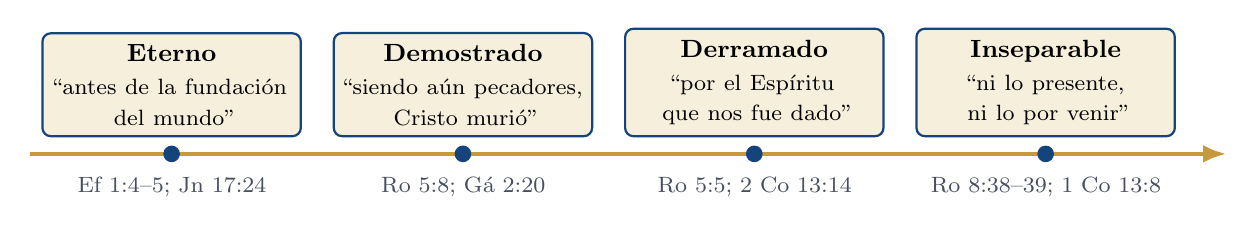
\begin{tikzpicture}[font=\small]
 \tikzset{hito/.style={draw=azul,line width=0.8pt,fill=papiro,rounded corners=3pt,text width=3.0cm,align=center,inner sep=4pt}}
 \draw[-{Latex[length=3mm]},dorado,line width=1.6pt] (0,0) -- (15.2,0);
 \foreach \x/\t/\r/\p in {0.9/Eterno/{antes de la fundación del mundo}/{Ef 1:4--5; Jn 17:24},
                          4.6/Demostrado/{siendo aún pecadores, Cristo murió}/{Ro 5:8; Gá 2:20},
                          8.3/Derramado/{por el Espíritu que nos fue dado}/{Ro 5:5; 2 Co 13:14},
                          12.0/Inseparable/{ni lo presente, ni lo por venir}/{Ro 8:38--39; 1 Co 13:8}} {
   \fill[azul] (\x+0.9,0) circle (3pt);
   \node[hito,above=6pt] at (\x+0.9,0) {\textbf{\t}\\[1pt]{\footnotesize ``\r''}};
   \node[below=5pt,text width=3.0cm,align=center,font=\footnotesize\color{gris}] at (\x+0.9,0) {\p};
 }
\end{tikzpicture}\par
{\footnotesize\color{gris}\textit{Figura 2.} El amor de Dios en Pablo: de antes del tiempo a más allá de la muerte. \textit{Nota.} Elaboración propia.}
\end{center}

\subsection{``El cual me amó y se entregó a sí mismo por mí''}
El amor eterno y soberano de Dios por un pueblo se vuelve, en Pablo, amor dirigido a una persona:

\begin{cita}Con Cristo estoy juntamente crucificado, y ya no vivo yo, mas vive Cristo en mí; y lo que ahora vivo en la carne, lo vivo en la fe del Hijo de Dios, el cual me amó y se entregó a sí mismo por mí.\fuente{(Gá 2:20)}\end{cita}

\begin{filologia}[Gá 2:20]
\begin{tabular}{@{}L{3.6cm}L{1.6cm}L{9.6cm}@{}}
\grc{τοῦ ἀγαπήσαντός με} & \grc{ἀγαπάω} & ``que me amó'': aoristo, un acto concreto en la historia. Singular: Pablo, que había perseguido a la iglesia (Gá 1:13), se sabe amado en persona. \\[2pt]
\grc{παραδόντος ἑαυτόν} & \grc{παραδίδωμι} & ``que se entregó a sí mismo'': el amor no da algo, se da. El mismo verbo describe al Padre que ``entregó'' al Hijo (Ro 8:32). \\
\end{tabular}
\end{filologia}

Pablo dice lo mismo del amor de Cristo por la iglesia, y lo dice con la imagen de Oseas: ``Maridos, amad a vuestras mujeres, así como Cristo amó a la iglesia, y se entregó a sí mismo por ella'' (Ef 5:25). El profeta compró a una esposa infiel (Os 3:1--2); Cristo se entregó por una esposa que no era santa, para hacerla santa (Ef 5:26--27).

\begin{nota}[Precisión]
Pablo no cita Oseas en Efesios 5; su texto explícito es Gn 2:24 (Ef 5:31). La relación con Oseas 3 es una lectura tipológica propia de esta serie, apoyada en que Pablo sí cita Oseas para hablar del amor que llama ``amada'' a la que no lo era (Ro 9:25; Os 2:23).
\end{nota}

\subsection{Los tres rasgos en Pablo}
\subsubsection*{Eterno}
``Según nos escogió en él antes de la fundación del mundo\ldots{} en amor habiéndonos predestinado'' (Ef 1:4--5). Pablo llama a los tesalonicenses ``hermanos amados por el Señor'', escogidos ``desde el principio'' (2 Ts 2:13), y bendice a ``Dios nuestro Padre, el cual nos amó y nos dio consolación eterna'' (2 Ts 2:16). Un amor anterior al tiempo produce una consolación que no se agota.

\subsubsection*{Soberano}
``Pero Dios, que es rico en misericordia, por su gran amor con que nos amó, aun estando nosotros muertos en pecados, nos dio vida juntamente con Cristo (por gracia sois salvos)'' (Ef 2:4--5). La única causa que el texto nombra es ``su gran amor'' (\grc{διὰ τὴν πολλὴν ἀγάπην αὐτοῦ}). Tito lo dice con otra palabra: ``cuando se manifestó la bondad de Dios nuestro Salvador, y su amor para con los hombres (\grc{φιλανθρωπία}), nos salvó, no por obras de justicia que nosotros hubiéramos hecho'' (Tit 3:4--5).

\subsubsection*{Inmutable}
``Nada nos podrá separar'' (Ro 8:39) es la versión paulina de ``yo \SENOR{} no cambio; por esto, hijos de Jacob, no habéis sido consumidos'' (Mal 3:6). Y en el himno al amor, Pablo atribuye al amor lo que Malaquías había dicho de Dios: ``El amor nunca deja de ser'' (\grc{ἡ ἀγάπη οὐδέποτε πίπτει}, 1 Co 13:8), mientras profecías, lenguas y ciencia habrán de acabarse.

\begin{center}\small\renewcommand{\arraystretch}{1.2}
\begin{tabular}{@{}L{2.2cm}L{4.2cm}L{4.2cm}L{4.2cm}@{}}
\toprule
\textbf{Rasgo} & \textbf{Escrituras de Israel} & \textbf{Pablo} & \textbf{Lo que muestra la cruz} \\ \midrule
Eterno & Jer 31:3; Os 11:1 & Ef 1:4--5; 2 Ts 2:13, 16 & El Hijo amado ``desde antes de la fundación del mundo'' es el que se entrega (Jn 17:24; Gá 2:20). \\
Soberano & Dt 7:7--8; 10:15; Mal 1:2; Os 14:4 & Ro 5:8; 9:13; Ef 2:4--5; Tit 3:4--5 & Cristo muere por débiles, impíos, pecadores y enemigos. \\
Inmutable & Mal 3:6; Os 11:8--9; Is 54:10; Cnt 8:7 & Ro 8:35--39; 1 Co 13:8 & Ni la muerte separa: el Amado resucitó y ``intercede por nosotros'' (Ro 8:34). \\
\bottomrule
\end{tabular}\par
{\footnotesize\color{gris}\textit{Tabla 6.} El amor eterno, soberano e inmutable, de Israel a Pablo. \textit{Nota.} Elaboración propia.}
\end{center}

\subsection{La plenitud del amor en Cristo}
``Para que, arraigados y cimentados en amor, seáis plenamente capaces de comprender con todos los santos cuál sea la anchura, la longitud, la profundidad y la altura, y de conocer el amor de Cristo, que excede a todo conocimiento, para que seáis llenos de toda la plenitud de Dios'' (Ef 3:17--19). Pablo ora por conocer lo que no se puede abarcar; Pink lo llama el amor ``infinito'' de Dios (Pink, 2020, p.~86). La oración desemboca en ``la plenitud de Dios'', la misma plenitud que ``habita corporalmente'' en Cristo (Col 2:9). Esa es la tesis de esta obra aplicada al amor: el amor que Dios es se ve entero en el Hijo, porque el Padre ama al Hijo desde siempre y en él ama a los suyos ``como también a mí me has amado'' (Jn 17:23).

%===================================================================
\section{Aplicación a la vida}

Juan extrae la consecuencia en una sola frase: ``Amados, si Dios nos ha amado así, debemos también nosotros amarnos unos a otros'' (1 Jn 4:11). El amor de Dios es incomunicable como fuente, pero se comunica como reflejo, y cada uno de sus rasgos encuentra un eco en la vida del creyente.

\subsection{Porque es eterno: seguridad}
Un amor que no empezó con la obediencia del creyente tampoco depende de su desempeño para continuar. ``En el amor no hay temor, sino que el perfecto amor echa fuera el temor'' (1 Jn 4:18). El creyente no sirve a Dios para ganar su amor; sirve porque ya es amado: ``Nosotros le amamos a él, porque él nos amó primero'' (1 Jn 4:19).

\subsection{Porque es soberano: humildad y gratitud}
Si Dios no amó a Israel por ser numeroso, ni a nosotros por ser buenos, nadie tiene de qué gloriarse: ``¿qué tienes que no hayas recibido? Y si lo recibiste, ¿por qué te glorías como si no lo hubieras recibido?'' (1 Co 4:7). El amor soberano enseña, además, a amar sin condiciones previas. Deuteronomio funda el mandamiento en el carácter de Dios, que ``ama también al extranjero dándole pan y vestido. Amaréis, pues, al extranjero; porque extranjeros fuisteis en la tierra de Egipto'' (Dt 10:18--19). Jesús lo lleva al extremo: ``Amad a vuestros enemigos\ldots{} para que seáis hijos de vuestro Padre que está en los cielos'' (Mt 5:44--45).

\subsection{Porque es inmutable: perseverancia en la prueba}
La disciplina no contradice el amor: ``el Señor al que ama, disciplina'' (He 12:6). Pink advierte que ningún cristiano debe dudar del amor de Dios cuando sufre, porque el Padre amaba al Hijo y no lo eximió del sufrimiento (Pink, 2020, p.~87). Ante la tribulación, la pregunta de Pablo no es ``¿por qué?'', sino ``¿quién nos separará?'' (Ro 8:35). Judas resume la tarea en tres palabras: ``conservaos en el amor de Dios'' (Jud 21). El amor no se gana, pero se habita.

\subsection{Amar como él}
El amor que se pide al creyente lleva la forma del amor de Dios: ``Sed, pues, imitadores de Dios como hijos amados. Y andad en amor, como también Cristo nos amó, y se entregó a sí mismo por nosotros'' (Ef 5:1--2). Pablo lo resume con la Torá, ``el cumplimiento de la ley es el amor'' (Ro 13:10), citando ``Amarás a tu prójimo como a ti mismo'' (Lv 19:18; Ro 13:9). Y en 1 Corintios 13 lo describe con rasgos que, leídos de nuevo, resultan ser los del amor de Dios: ``El amor es sufrido, es benigno\ldots{} no guarda rencor\ldots{} Todo lo sufre, todo lo cree, todo lo espera, todo lo soporta. El amor nunca deja de ser'' (1 Co 13:4--8).

\begin{center}\small\renewcommand{\arraystretch}{1.2}
\begin{tabular}{@{}L{2.4cm}L{5.4cm}L{7.0cm}@{}}
\toprule
\textbf{Rasgo} & \textbf{En Dios} & \textbf{Reflejo en el creyente} \\ \midrule
Eterno & Amó antes de que existiéramos (Jer 31:3; Ef 1:4) & Seguridad sin temor (1 Jn 4:18--19) \\
Soberano & Amó sin causa en nosotros (Dt 7:7--8; Ro 5:8) & Humildad (1 Co 4:7) y amor al que no lo merece (Dt 10:19; Mt 5:44) \\
Inmutable & No deja de amar (Mal 3:6; Ro 8:39) & Perseverancia en la prueba (Ro 8:35; Jud 21) y un amor que ``nunca deja de ser'' (1 Co 13:8) \\
\bottomrule
\end{tabular}\par
{\footnotesize\color{gris}\textit{Tabla 7.} Del amor de Dios al amor del creyente. \textit{Nota.} Elaboración propia.}
\end{center}

\subsection{Conclusión}
El verso que vertebra esta obra dice: ``alábese en esto el que se hubiere de alabar: en entenderme y conocerme, que yo soy \SENOR, que hago misericordia, juicio y justicia en la tierra; porque estas cosas quiero'' (Jer 9:24). Conocer a Dios como amor no es conocer un sentimiento; es conocer a una persona que ama desde siempre, sin causa fuera de sí y sin cambio. Ese amor se dejó ver en Moriah, en el Sinaí, en la casa de Oseas y, por último, en la cruz, donde el Padre ``no escatimó ni a su propio Hijo''. Por eso la confesión de Juan es también la de esta serie: ``nosotros hemos conocido y creído el amor que Dios tiene para con nosotros. Dios es amor'' (1 Jn 4:16).

%===================================================================
\section*{Referencias}
\refapa{Carson, D.~A. (2000). \emph{The difficult doctrine of the love of God}. Crossway.}
\refapa{Carson, D.~A. (2013). \emph{Falacias exegéticas}. Editorial CLIE.}
\refapa{Dunn, J.~D.~G. (1998). \emph{The theology of Paul the apostle}. Eerdmans.}
\refapa{Elliger, K., \& Rudolph, W. (Eds.). (1997). \emph{Biblia Hebraica Stuttgartensia} (5.ª ed.). Deutsche Bibelgesellschaft.}
\refapa{García Martínez, F. (1992). \emph{Textos de Qumrán}. Trotta.}
\refapa{Maimónides. (s.f.). \emph{Mishné Torá: Hiljot Teshuvá} [10:3]. Sefaria. https://www.sefaria.org}
\refapa{\emph{Misná: Berajot} [9:5]; \emph{Yadayim} [3:5]; \emph{Pirké Avot} [3:14; 5:16]. (s.f.). Sefaria. https://www.sefaria.org}
\refapa{Moo, D.~J. (1996). \emph{The epistle to the Romans}. Eerdmans.}
\refapa{Moran, W.~L. (1963). The ancient Near Eastern background of the love of God in Deuteronomy. \emph{Catholic Biblical Quarterly}, \emph{25}(1), 77--87.}
\refapa{Nestle, E., \& Aland, K. (Eds.). (2012). \emph{Novum Testamentum Graece} (28.ª ed.). Deutsche Bibelgesellschaft.}
\refapa{Pink, A. W. (2020). \emph{Los atributos de Dios} (E. Rodríguez Cruz, Trad.). Chapel Library. (Obra original publicada en 1930)}
\refapa{Rahlfs, A., \& Hanhart, R. (Eds.). (2006). \emph{Septuaginta} (Ed. rev.). Deutsche Bibelgesellschaft.}
\refapa{Rashi. (s.f.). \emph{Comentario a la Torá} [Dt 7:7] y \emph{Comentario al Cantar de los Cantares} [introducción]. Sefaria. https://www.sefaria.org}
\refapa{\emph{Santa Biblia: Reina-Valera 1960}. (1960). Sociedades Bíblicas en América Latina.}
\refapa{\emph{Shemot Rabá} [3:6]. (s.f.). Sefaria. https://www.sefaria.org}
\refapa{\emph{Sidur asquenazí: Ahavá rabbá; Ahavat olam}. (s.f.). Sefaria. https://www.sefaria.org}
\refapa{\emph{Sifré Devarim} [32]. (s.f.). Sefaria. https://www.sefaria.org}
\refapa{Steinsaltz, A. (Ed.). (2017). \emph{Koren Talmud Bavli: Edición William Davidson} [Berajot 11b, 61b; Julín 89a]. Sefaria. https://www.sefaria.org}
\refapa{Strong, J. (1890). \emph{The exhaustive concordance of the Bible}. Hunt \& Eaton.}
\refapa{\emph{Targum Ónkelos} [Dt 6:5]. (s.f.). Sefaria. https://www.sefaria.org}
\refapa{Vermes, G. (2004). \emph{The complete Dead Sea Scrolls in English} (Ed. rev.). Penguin.}
\refapa{Vine, W.~E. (1999). \emph{Diccionario expositivo de palabras del Antiguo y del Nuevo Testamento exhaustivo}. Caribe.}

\end{document}
